\documentclass[pdflatex,compress,mathserif]{beamer}

%\usetheme[dark,framenumber,totalframenumber]{ElektroITK}
\usetheme[darktitle,framenumber,totalframenumber]{ElektroITK}

\usepackage[utf8]{inputenc}
\usepackage[T1]{fontenc}
\usepackage{lmodern}
\usepackage[bahasai]{babel}
\usepackage{amsmath}
\usepackage{amsfonts}
\usepackage{amssymb}
\usepackage{graphicx}
\usepackage{multicol}
\setbeamertemplate{caption}[numbered]

\newcommand*{\Scale}[2][4]{\scalebox{#1}{$#2$}}%

\title{MATRIKULASI}
\subtitle{MATEMATIKA DASAR}

\author{Mifta Nur Farid}

\begin{document}

\maketitle

\section{Pengantar}

	\subsection{Perkenalan Diri}
		\begin{frame}{Perkenalan Diri}
			\begin{multicols}{2}
				\begin{center}
					
\includegraphics[width=0.7\linewidth]{pict/00}
				\end{center}
				\begin{itemize}
					\item Mifta Nur \textbf{Farid}
					\item Dosen Teknik Elektro
					\item Probolinggo, Surabaya, Balikpapan
					\item Mendaki Gunung, Bermain Games, Nonton Film
				\end{itemize}
				\columnbreak
			\end{multicols}
		\end{frame}
	
	\subsection{Pokok Bahasan}
		\begin{frame}{Pokok Bahasan}
			\begin{multicols}{2}
				\begin{enumerate}
					\item Pertidaksamaan Linier
					\begin{itemize}
						\item Interval
						\item Penyelesaian Pertidaksamaan
					\end{itemize}
					\item Fungsi dan Limit
					\begin{itemize}
						\item Fungsi
						\item Limit
					\end{itemize}
					\item Trigonometri
					\item Turunan
					\item Integral
					\begin{itemize}
						\item Integral Tak Tentu
						\item Integral dengan Substitusi
						\item Integral Tentu
					\end{itemize}
				\end{enumerate}
			\end{multicols}
		\end{frame}

\section{Pertidaksamaan Linier}

	\subsection{Interval}

		\begin{frame}
			\frametitle{Pertidaksamaan}
			\begin{itemize}
				\item Pertidaksamaan:
				\begin{equation}
					5x - 4 > 2x + 3
				\end{equation}
				\item Persamaan menggunakan simbol $ = $
				\item Pertidaksamaan menggunakan simbol
				\begin{center}
					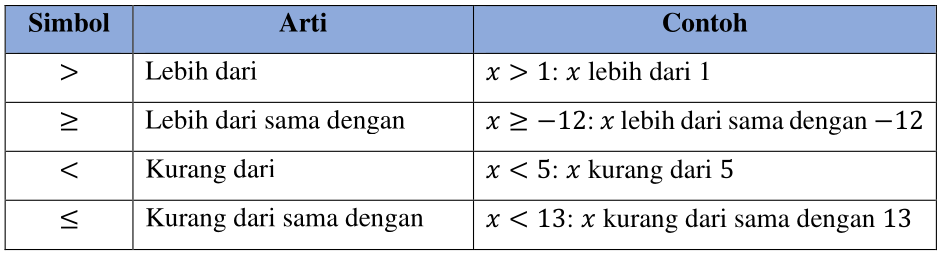
\includegraphics[width=\linewidth]{pict/01}
				\end{center}
			\end{itemize}
		\end{frame}
	
		\begin{frame}{Pertidaksamaan}
			\begin{itemize}
				\item Penyelesaian persamaan
				\begin{align*}
					5x - 4 &= 2x + 3\\
					5x - 2x &= 3 + 4\\
					3x &= 7\\
					x &= \frac{7}{3}
				\end{align*}
				\item Penyelesaian pertidaksamaan: rentang atau nilai variabel yang tidak diketahui yang memenuhi pertidaksamaan
			\end{itemize}
		\end{frame}
	
		\begin{frame}{Interval}
			\begin{itemize}
				\item Himpunan penyelesaian suatu pertidaksamaan dinyatakan dalam notasi himpunan atau bentuk selang atau \textit{interval}
				\item Jenis-jenis selang
				\begin{enumerate}
					\item Selang berhingga dan tertutup
					\item Selang berhingga dan terbuka
					\item Selang berhingga dan setengah terbuka atau setengah tertutup
					\item Selang tak hingga dan tertutup
					\item Selang tak hingga dan terbuka
					\item Selang tak hingga, terbuka, dan tertutup
				\end{enumerate}
			\end{itemize}
		\end{frame}
	
		\begin{frame}
			\frametitle{Selang berhingga dan tertutup}
			\begin{itemize}
				\item Notasi: $ [a,b] $
				\item Dinyatakan dalam notasi himpunan:
				\begin{equation}
					\{x:a \leq a \leq b\}
				\end{equation}
				\item Grafik selang:
				\begin{figure}
					\centering
					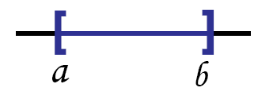
\includegraphics[width=0.5\linewidth]{pict/02}
					\caption{Grafik selang $[a,b]$}
					\label{fig:02}
				\end{figure}
			\end{itemize}
		\end{frame}
	
		\begin{frame}
			\frametitle{Selang berhingga dan terbuka}
			\begin{itemize}
				\item Notasi: $ (a,b) $
				\item Dinyatakan dalam notasi himpunan:
				\begin{equation}
					\{x:a < a < b\}
				\end{equation}
				\item Grafik selang:
				\begin{figure}
					\centering
					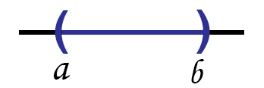
\includegraphics[width=0.5\linewidth]{pict/03}
					\caption{Grafik selang $(a,b)$}
					\label{fig:03}
				\end{figure}
			\end{itemize}
		\end{frame}
	
		\begin{frame}
			\frametitle{Selang berhingga dan setengah terbuka atau setengah tertutup}
			\begin{itemize}
				\item Notasi: $ (a,b] $ atau $ [a,b) $
				\item Notasi himpunan:
				\begin{align*}
					\text{Jika notasi } (a,b]& \text{, maka notasi himpunan }\{x:a < a \leq b\} \\
					\text{Jika notasi } [a,b)& \text{, maka notasi himpunan }\{x:a \leq a < b\} \\
				\end{align*}
				\item Grafik selang:
				\begin{multicols}{2}
					\begin{figure}
						\centering
						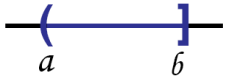
\includegraphics[width=0.5\linewidth]{pict/04}
						\caption{Grafik selang $(a,b]$}
						\label{fig:04}
					\end{figure}
					\columnbreak
					\begin{figure}
						\centering
						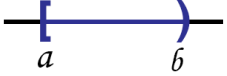
\includegraphics[width=0.5\linewidth]{pict/05}
						\caption{Grafik selang $[a,b)$}
						\label{fig:05}
					\end{figure}
				\end{multicols}
			\end{itemize}
		\end{frame}

	\subsection{Penyelesaian Pertidaksamaan}

\section{Fungsi Dan Limit}

	\subsection{Fungsi}

	\subsection{Limit}

\section{Trigonometri}

\section{Turunan}

\section{Integral}

	\subsection{Integral Tak Tentu}

	\subsection{Integral dengan Substitusi}
	
	\subsection{Integral Tentu}

\end{document}
